\chapter{Experiments}
\label{chap:experiments}

The goal of our work is to compare two implementations of the Speed layer, one using Storm and another using Spark Streaming.
We evaluate both approaches from two sides.
First, we measure the performance of the system to detect which techology allows to process more events for the specified time interval.
Second, we compare the codability of these variants.
Using the obtain results, we make a choice which technology fits better our case.

Performance evaluation

Figure~\ref{fig:test_system_parameters} represents the parmeters of the test system.
For the simplicity of testing we use only one machine.
To obtain more reliable results one should also run these systemts on a cluster of several machines.

\begin{figure}
  \centering
  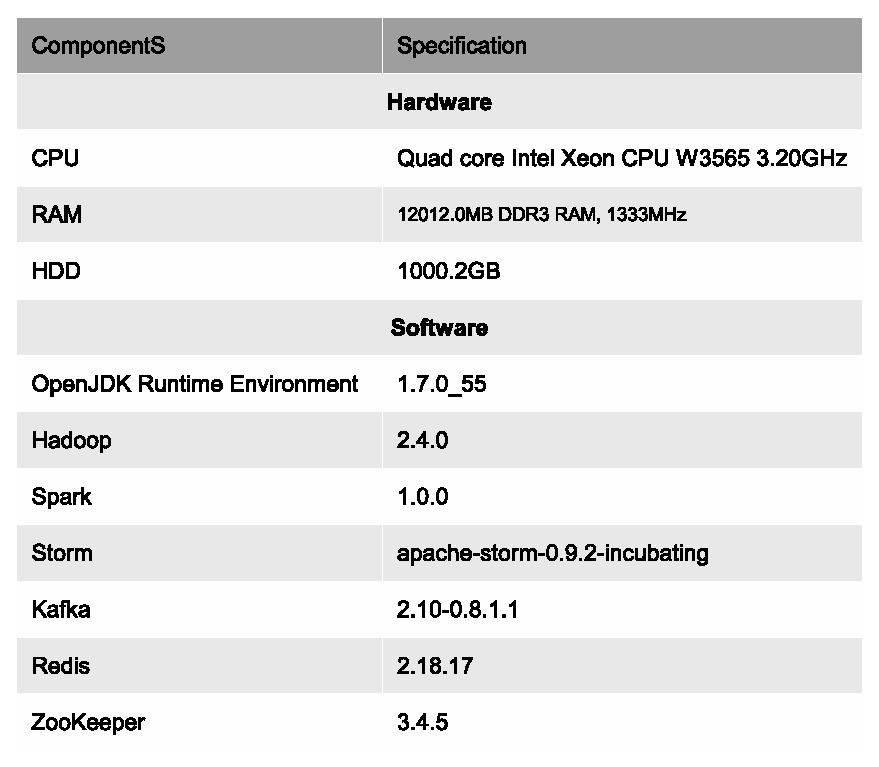
\includegraphics [width=0.9\textwidth]{images/test_system_parameters}
  \caption{Test system parameters}
  \label{fig:test_system_parameters}
\end{figure}

As an input, we use automatically generated events, that imitate the real data flow.
To make the comparison more objective, we vary the number of processed messages.
In our tests we use three sets: 1000 events, 10,000 events and 100,000 events.
Each of these sets contains all types of events mentioned in Chapter % TODO.
The values of event parameters are generated randomly.

As an output, we obtain the speed of event processing.
We measure how many events the system processes per second and compare these figures for both Storm and Spark implementations. 

\begin{figure}
  \centering
  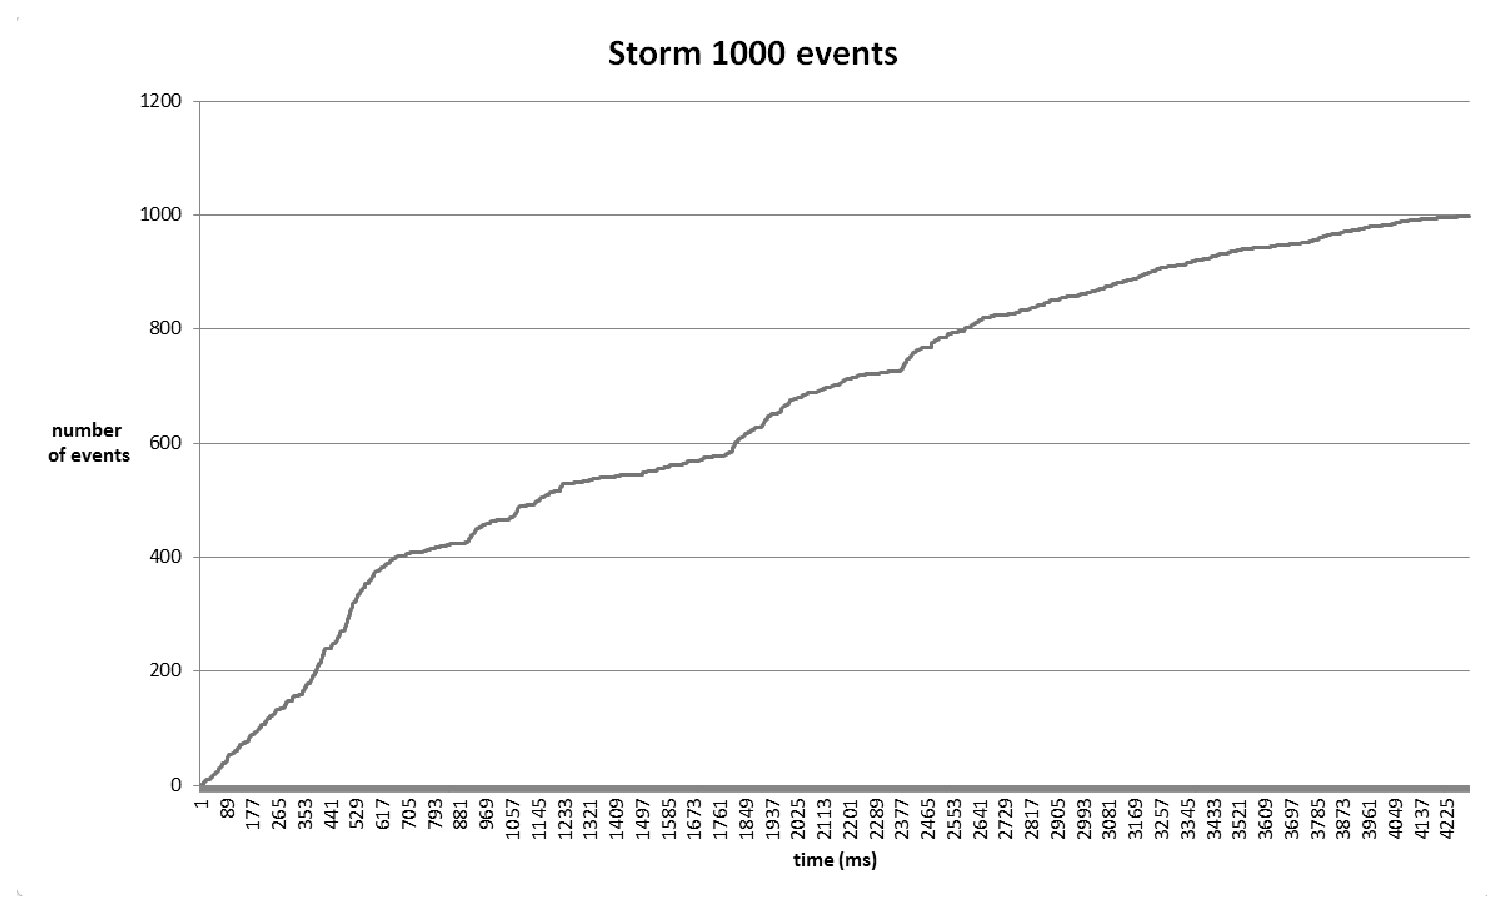
\includegraphics [width=1.0\textwidth]{images/storm1000}
  \caption{Storm 1000}
  \label{fig:storm1000}
\end{figure}

\begin{figure}
  \centering
  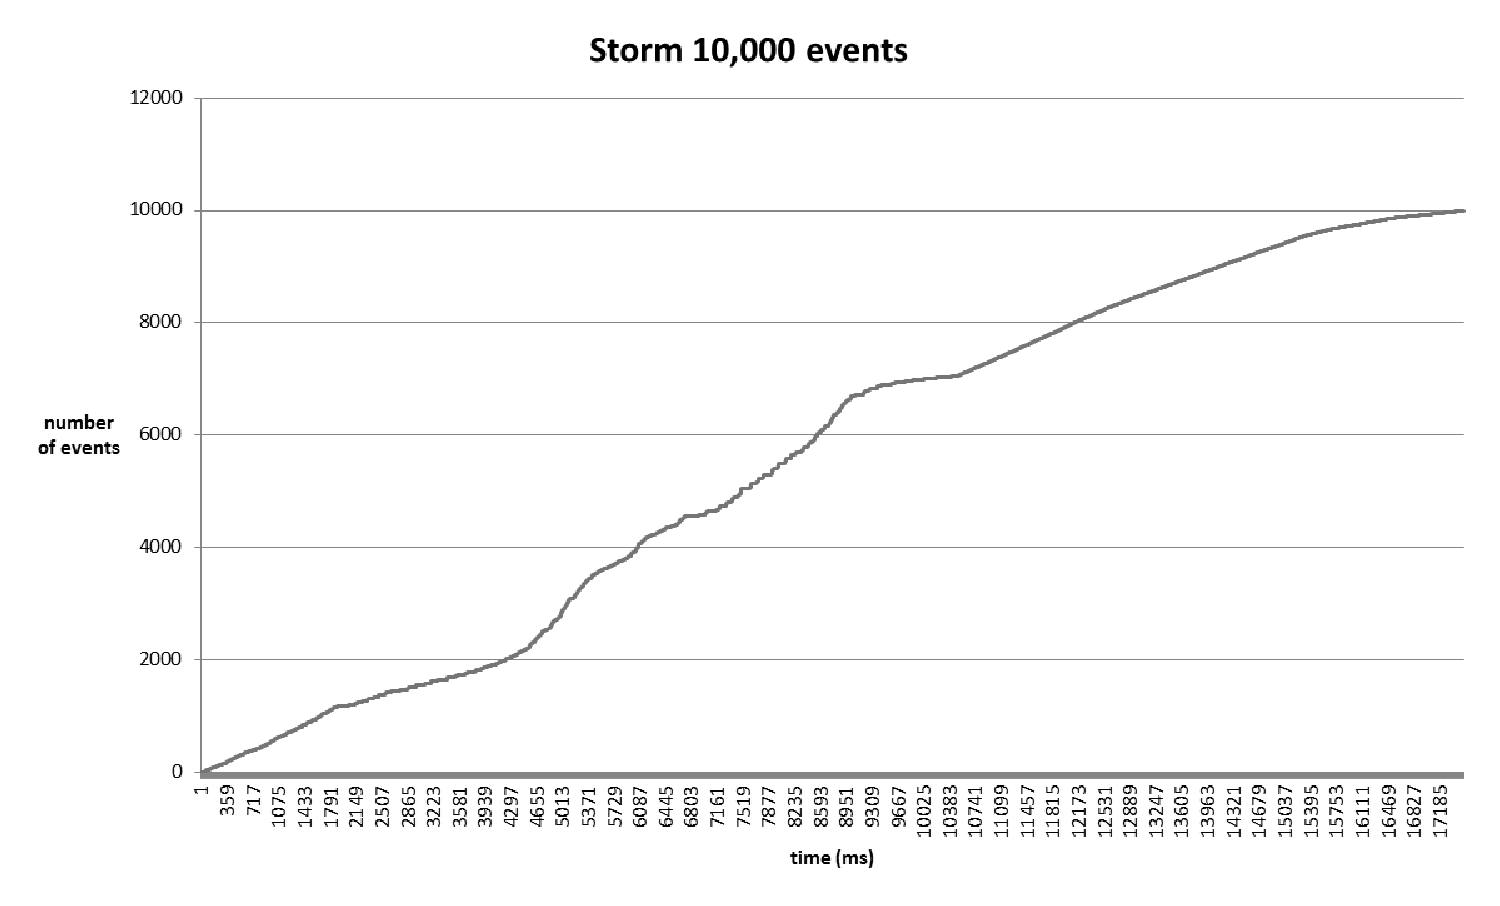
\includegraphics [width=1.0\textwidth]{images/storm10000}
  \caption{Storm 10000}
  \label{fig:storm10000}
\end{figure}

\begin{figure}
  \centering
  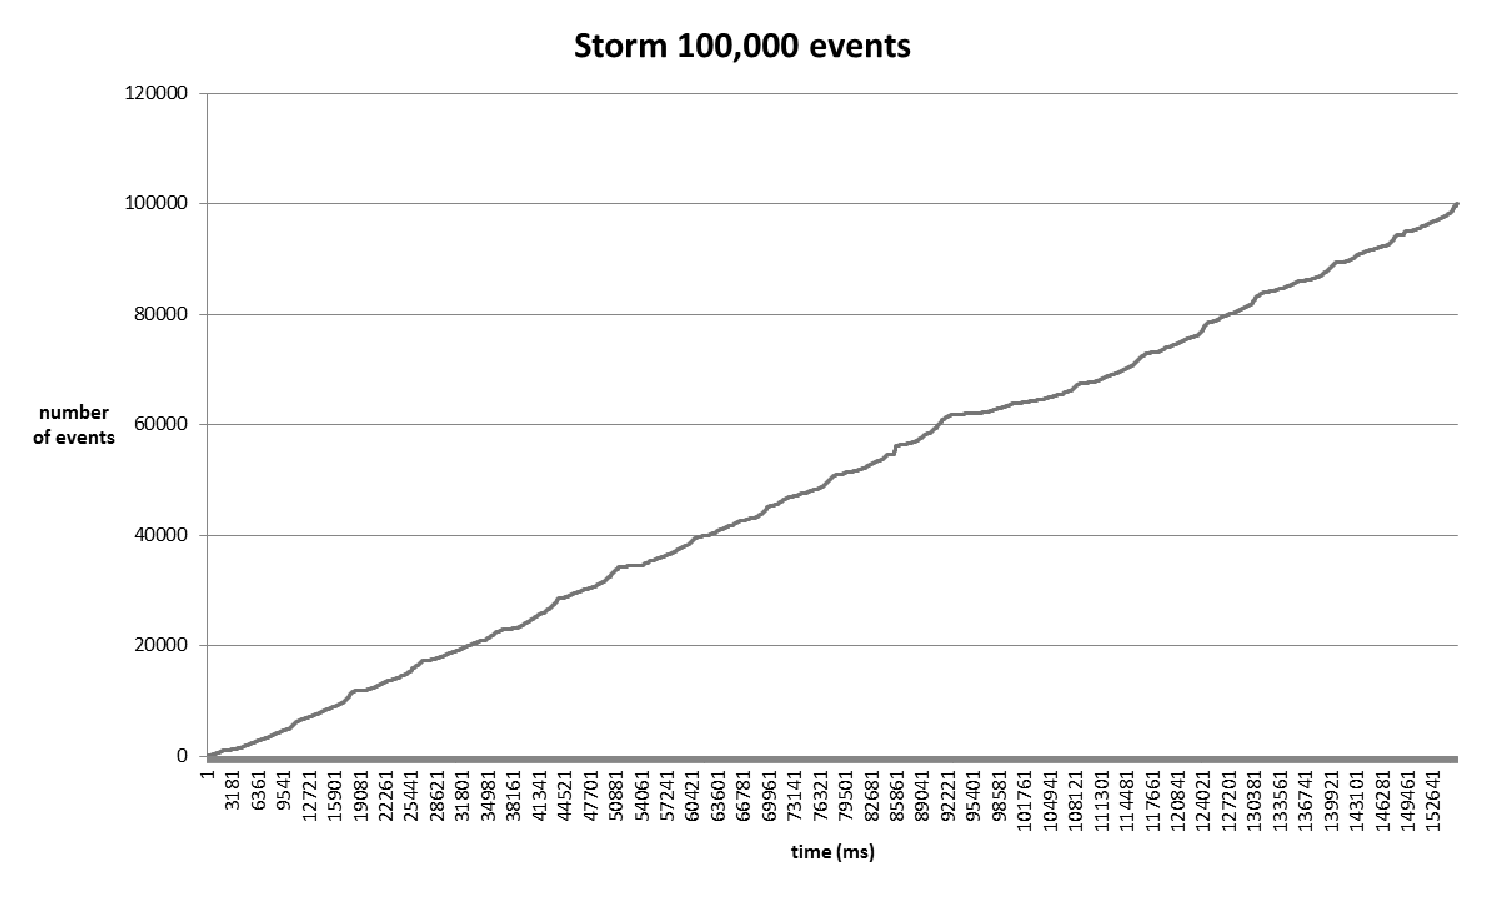
\includegraphics [width=1.0\textwidth]{images/storm100000}
  \caption{Storm 100000}
  \label{fig:storm100000}
\end{figure}

\begin{figure}
  \centering
  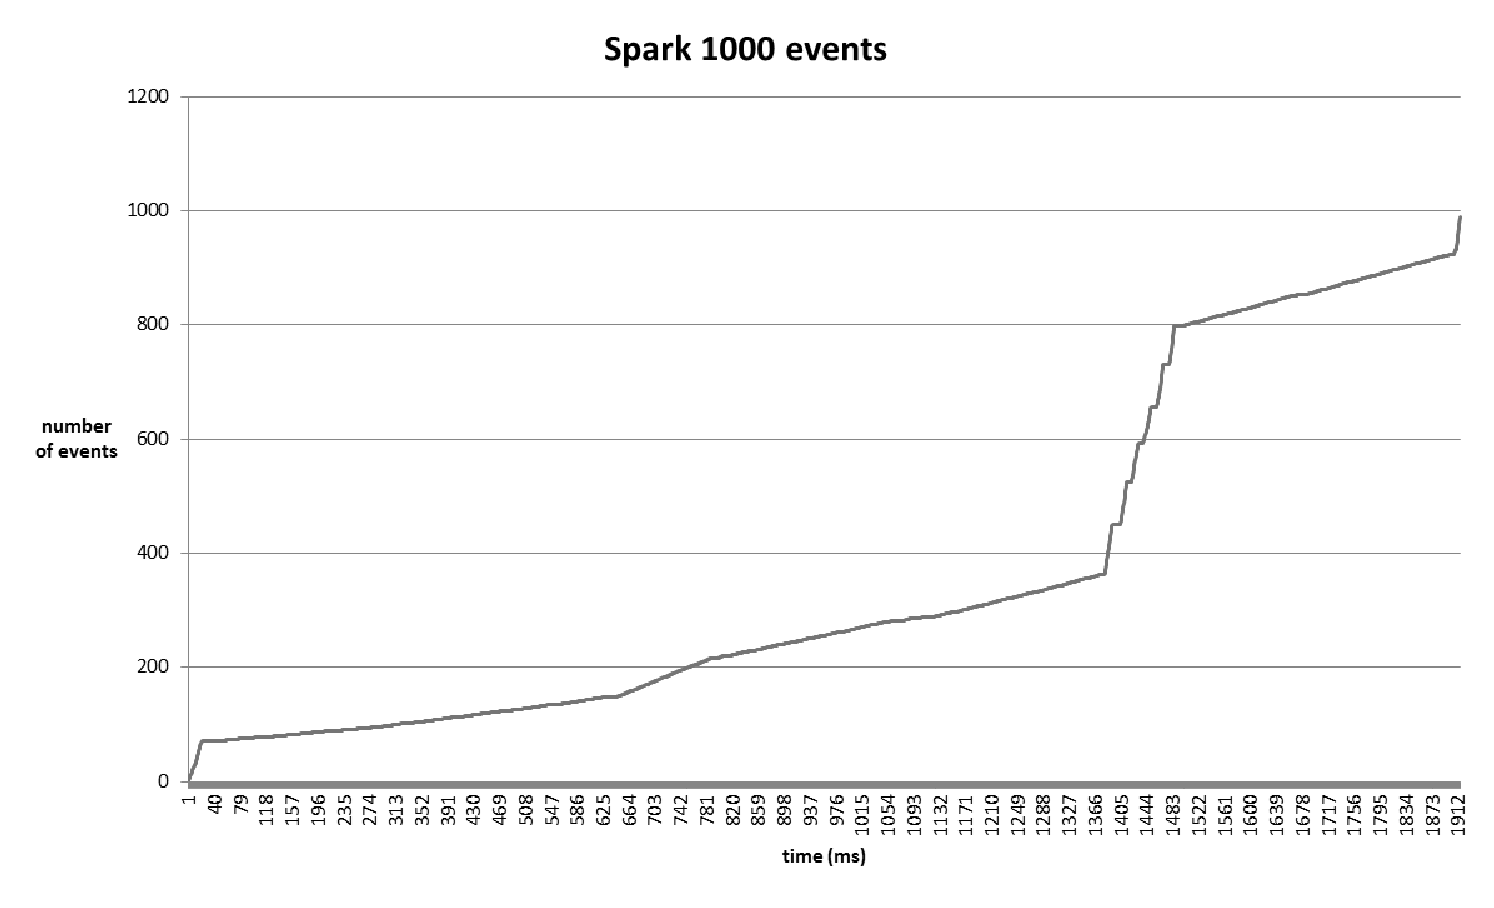
\includegraphics [width=1.0\textwidth]{images/spark1000}
  \caption{Spark 1000}
  \label{fig:spark1000}
\end{figure}

\begin{figure}
  \centering
  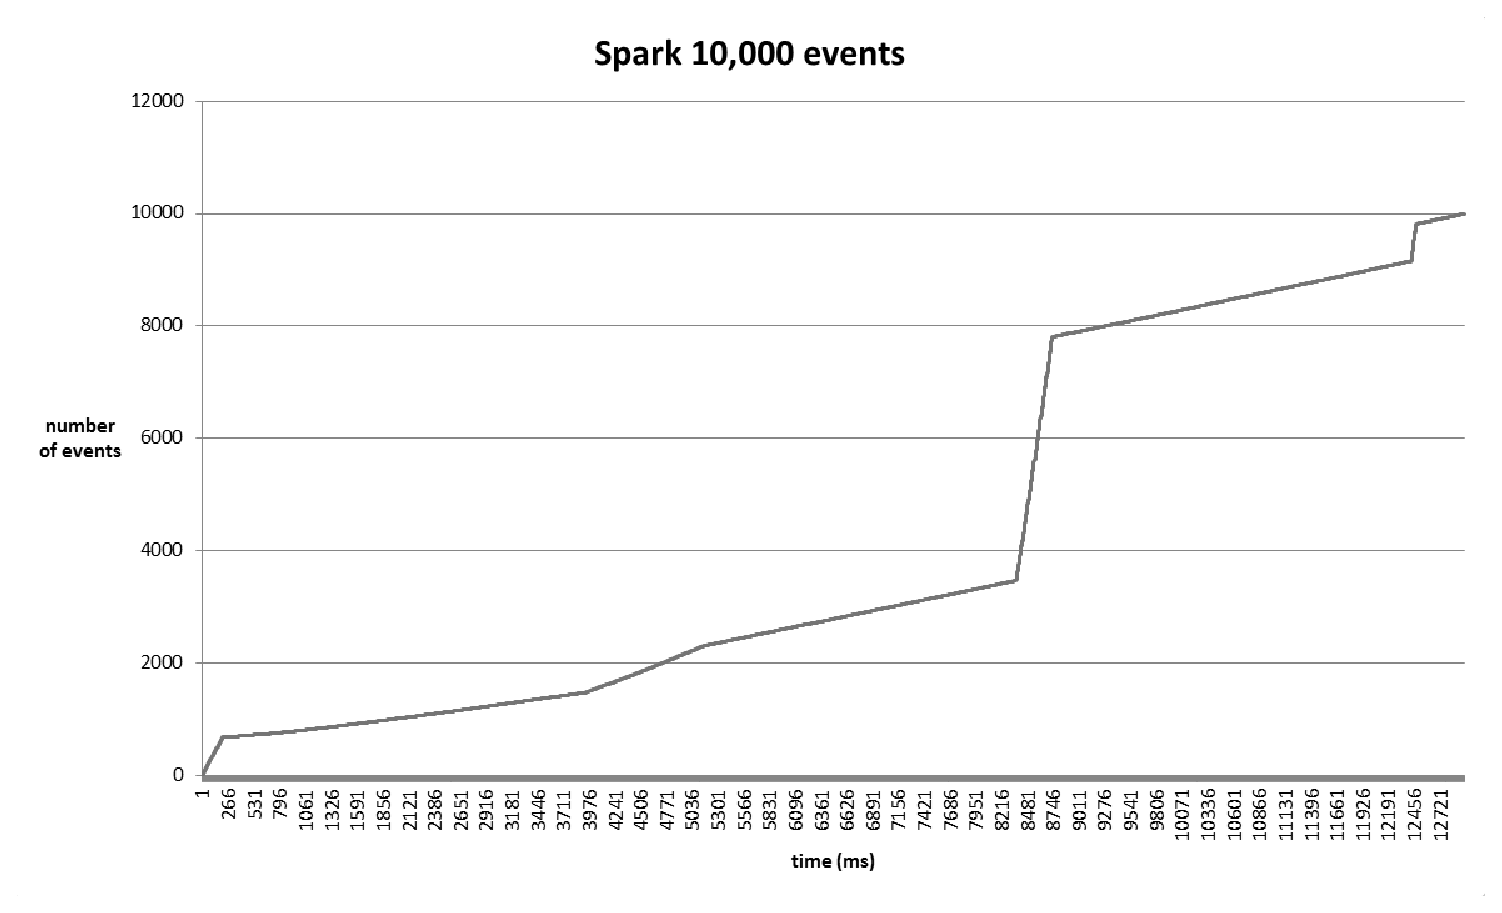
\includegraphics [width=1.0\textwidth]{images/spark10000}
  \caption{Spark 10000}
  \label{fig:spark10000}
\end{figure}

\begin{figure}
  \centering
  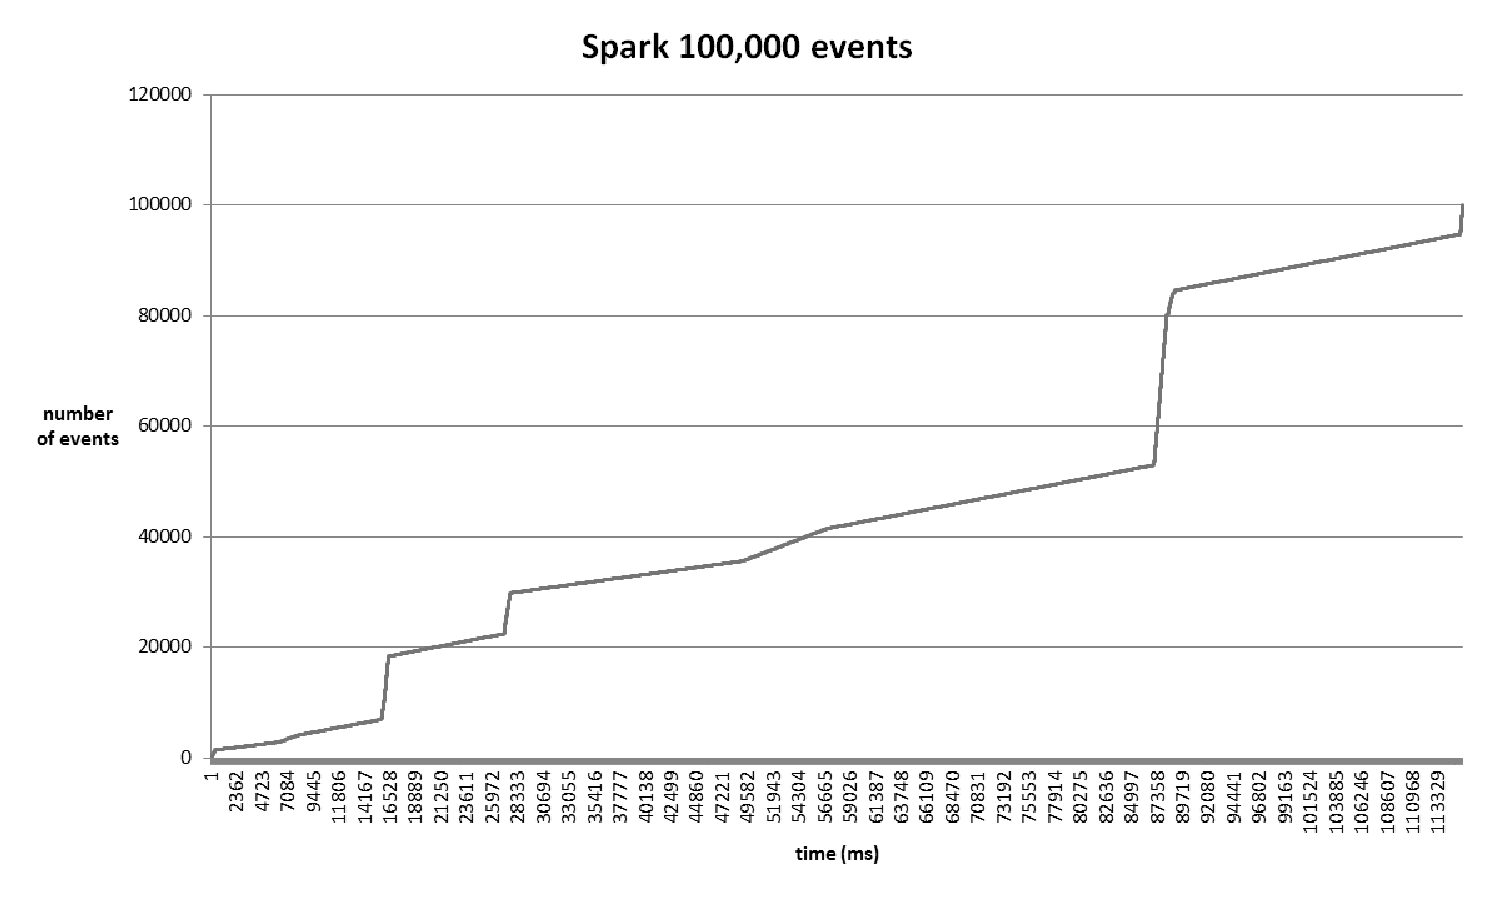
\includegraphics [width=1.0\textwidth]{images/spark100000}
  \caption{Spark 100000}
  \label{fig:spark100000}
\end{figure}



% machines we use, parameters we set, parameters we want observe - for performance
% number of client, number of messages

% measure: latency, cpu overhead. Can be dependent on batch size in Batch layer

It should be mentioned that they solve a bit different problems.
Storm performs indeed a real time processing.
Spark, in its turn, does a micro-batching.
In the latter case the size of batch is small, so this technology can be considered close to real time processing.
Spark has latency

Codability comparison

In the previous section Storm and Spark implementations are compared from the performance point of view.
However, it is not the decisive factor when choosing which technology to use in our project.
In modern world the cost of hardware decreases significantly comparing to the prices that were ten years ago.
Thus it is not a problem to add several machines into our cluster, increasing performance.
Hence the human sources become an important factor for making our choice.
In this section we compare which technology, Storm or Spark, is easier to implement.

\mnote{installation}
The installation process of Storm is a bit more complicated than the installation of Spark.
Storm requires two additional tools to be installed on a machine.
First, it needs ZooKeeper for coordinating the cluster.
Second, Strom should run under supervision, so a supervisor service like a \textit{supervisord} is needed.
From the practical side we had some difficulties with combining the versions of these software tools to make them interact properly.
Spark, in its turn, only requires a Spark assembly in the CLASSPATH.

\mnote{configuration}
Storm and Spark have different configuration settings to integrate with Kafka.
To allow Kafka-Storm interaction, we use an existing storm-kafka module.
It provides a special class \textit{KafkaSpout}, that receives data from Kafka.
As Kafka and Storm interact through ZooKeeper, we specify ZooKeeper hosts, port and a path to Kafka brokers (clusters).
Furthermore, each Kafka spout stores consumer offsets in ZooKeeper.
For this purpose we specify a root path in ZooKeeper and a unique id for every spout.
There is a possibility to set from which offset to start consuming.
Also we indicate a topic name for each spout.

Similar to the Storm case, with Spark we create one DStream for each Kafka topic.
Because of this we have a possibility to handle each type of events separately.
In Storm we run a Topology, here we run a StreamingContext.
To provide it with the data from Kafka, the following settings are needed.
We specify a list of ZooKeeper hosts, the name of Kafka consumer group and the topic name.
The number of threads used for consuming data from a Kafka topic is also customizable.

\mnote{usage}

\mnote{documentation}
Both Spark and Storm have an official online documentation available.
They have a good description of the general usage.
The Storm website provides a link to an example project named \textit{storm-starter} that can be used as a basis for creating your own project.
Spark package also contains an example project, that includes \textit{JavaKafkaWordCount.java} code, that can be used as a starting point. 
The only distinction that should be mentioned is the availability of documentation about integration with Kafka.
As the support of Kafka was included only in the last version of Storm (storm-kafka-0.9.2-incubating), this module is not wholly documented and there are no examples on the official Storm site.
On the contrary, Spark has an example code on its official site and API documentation. 

\mnote{community size}
Another important factor is a community size of the project.
Documentation is a good source of information, however in cannot cover all the questions that can appear during the development process.
People who work on a project are the most competent sources, they can answer unusual questions and help providing code examples.
Moreover, they can determine that the unexpected behavior of the system is a bug and promote a solution.
We can compare the number of contributors of Spark and Storm using github statistics, because both these projects present there.
Currently Spark has 355 contributors, while Storm has 115 contributors. 

% paragraph about installation
% about syntax (Storm close to MapReduce)
% about debagging
% paragraph about documentation
% about maintainance - monitor the software, restart after failure, etc

% TODO: installation of Storm and Spark on the machine


% move to another part

% kafka has to be adopted to spark or to storm independently
\mnote{Compatibility with Kafka}
We use Kafka as a message queue in the backend part of the Menthal project.
Therefore it is needed to adjust necessary setting to allow Storm or Spark receive messages from Kafka topics.
Currently for each event type we use a separate Kafka topic.
For now there are 9 of them: app\_install, app\_session, call\_missed, call\_outgoing, call\_received, screen\_off, screen\_unlock, sms\_received and sms\_sent.  
In the future this list can be changed or extended.
Moreover, the event type detection can be done in different way.
For instance, the information about the event type can be carried in a message header.
However, currently the infrastructure of our project is constructed in a way that the message type is determined by the Kafka topic it goes from.

% assume that we alreadu know about topologies and so on
\mnote{Kafka and Strom}
In Storm all the logic is based on the computation graph named \textit{Topology}.
It consists of \textit{Spouts}, the sources of data and \textit{Bolts}, data consumers.
In our project we have a single topology that contains one spout and one bolt for each Kafka topic.
% part of implementation:
To allow Kafka-Storm interaction, we use an existing storm-kafka module.
It provides a special class \textit{KafkaSpout}, that receives data from Kafka.
As Kafka and Storm interact through ZooKeeper, we specify ZooKeeper hosts, port and a path to Kafka brokers (clusters).
Furthermore, each Kafka spout stores consumer offsets in ZooKeeper.
For this purpose we specify a root path in ZooKeeper and a unique id for every spout.
There is a possibility to set from which offset to start consuming.
Also we indicate a topic name for each spout.
There are some other settings that allow to adjust the Kafka-Storm interaction more precisely, that are not mentioned in our work.

\mnote{Kafka and Spark}
% the same problem
Spark has another conception, different from Storm.
In our project we use Spark Streaming - technology that allows to handle data in real time.
Thus the main notion in Spark implementation is a \textit{discretized stream} (DStream).
Later on this stream is divided inro batches and they are processed by a Spark engine.
Similar to the Storm case, we also create one DStream for each Kafka topic.
Because of this we have a possibility to handle each type of events separately.
In Storm we run a Topology, here we run a StreamingContext.
To provide it with the data from Kafka, the following settings are needed.
We specify a list of ZooKeeper hosts, the name of Kafka consumer group and the topic name.
The number of threads used for consuming data from a Kafka topic is also customizable.
Not all the possible setting are mentioned here.

As a result, we can note that both Spark and Storm have built-in modules to interact with Kafka.
Moreover, the needed setting are almost the same and do not present any difficulties.


\mnote{Usage}
As regards the usability, Storm seems to be more intuitive than Spark Streaming.
It was mentioned that Storm consists of spouts and bolts.
We receive the data from Kafka spout.
So, the only thing we have to implement is one or several bolts that process the received information.
In our simple case we use only one bolt, that inherits \textit{BaseRichBolt}.
We override its \textit{execute} method to perform our operations.

In the case of Spark Streaming, we have to deal with its Resilient Distributed Datasets (RDD).
RDD represents the Spark (not Spark Streaming) main concept, that allows to perform batch processing.
To provide near real-time processing, Spark Streaming uses DStreams as sources of data.
Each DStream than divided by Spark into a sequence of RDDS.
From this moment Spark can perform the same operations on RDDs as it uses in batch processing.
In our case we use \textit{foreachRDD} as an output operation on RDDs.
This function triggers the computation of the corresponding stream.
RDD is a distributed collection, and to execute a peace of code, the Spark driver node serializes this code and sends to the workers, where it can be deserialized and executed.
Our problem is that we use several classes to process the input data and store the results in Redis, that are not serializable.
Therefore we have to be careful with the place where the code, that calls the functions from nonserializable classes, is placed.
The best solution in our case is to use \textit{foreachPartition} method, that is called for each RDD.
As a result, we create an instance of this nonserializable class for the whole partition and than apply the needed operations on each record of this partition. 
 
\mnote{Redis}
The finishing point of both Storm and Spark approaches is calculating aggregations on the received data and storing the results into a database (Redis).
There is nothing to compare in this case, because both of these technologies use exactly the same code to perform these steps.

% TODO: scaling of Storm and Kafka on several nodes


\authorsection{Evaluation of possibilities of the system}{NO}